\chapter{Identification of hydrodynamic coefficients}
\label{app:damping}

\section{Purpose}
The purpose with this test is to
identify the hydrodynamic coefficients used in the linear model for
AAUSHIP, being the hydrodynamic damping coefficients for the 5 \ac{DOF} damping
matrix~\vref{eq:damping-matrix} and the restoring force during pitch and roll. This is accomplished by
three sea trails; a surge test, a sway test and a yaw
test, performed in a lake, and two tests to determine pitch and roll, performed in a small pool.

\section{Theory}
The surge, sway and yaw tests are performed with theory of one method of testing, and theory of another method is used when determining pitch and roll. The damping in surge, sway and yaw is estimated by fitting data to a first order differential equation where the pitch and roll dampings are determined from fitting onto a second order differential equation. These two ways of determining the damping coefficients will be denoted \textit{method one} for the first order fitting and \textit{method two} for the second order fitting.

\subsection{Which parameters to determine}
The parameters that needs to be determined is the damping coefficients
from the damping matrix. The 5 \ac{DOF} damping matrix is reduced from the 6 \ac{DOF} damping matrix from \ref{eq:6dofd}:
\begin{align}
D = -
\begin{bmatrix}
X_u & 0 & 0 & 0 & 0\\
0 & Y_v & Y_p & 0 & Y_r\\
0 & K_v & K_p & 0 & K_r\\
0 & 0 & 0 & M_q & 0\\
0 & N_v & N_p & 0 & N_r
\end{bmatrix}
\end{align}
and the coefficients from the restoring force matrix $G$, \ref{eq:restoreforce}, being:
\begin{align}
G = -
\begin{bmatrix}
0 & 0 & 0 & 0 & 0\\
0 & 0 & 0 & 0 & 0\\
0 & 0 & K_\varphi & 0 & 0\\
0 & 0 & 0 & M_\theta & 0\\
0 & 0 & 0 & 0 & 0
\end{bmatrix}
\end{align}
The different coefficients can be found by writing the complete dynamic system:
\begin{align}
M_{RB} \dot \nu + D\nu + G\eta = \tau
\end{align}
where:
\begin{align}
\nu =
\begin{bmatrix}
u & v & p & q & r
\end{bmatrix}^T
\quad , \quad
\eta =
\begin{bmatrix}
x & y & \varphi & \theta & \psi
\end{bmatrix}^T
\end{align}
and
\begin{align}
M_{RB} =
\begin{bmatrix}
m & 0 & 0 & mz_g & -my_g\\
0 & m & -mz_g & 0 & mx_g\\
0 & -mz_g & I_x & -I_{xy} & -I_{xz}\\
mz_g & 0 & -I_{yx} & I_y & -I_{yz}\\
-my_g & mx_g & -I_{zx} & -I_{zy} & I_z
\end{bmatrix}
\end{align}
The full 5 \ac{DOF} dynamic system equations can then be written as:
\begin{align}
M_{RB1}\dot \nu + D_{1} \nu &= \tau\\
M_{RB2}\dot \nu + D_{2} \nu &= \tau\\
M_{RB3}\dot \nu + D_{3} \nu + G_{3} \eta &= \tau\\
M_{RB4}\dot \nu + D_{4} \nu + G_{4} \eta &= \tau\\
M_{RB5}\dot \nu + D_{5} \nu &= \tau
\end{align}
%Which can be outlined as:
%\begin{align}
%\begin{bmatrix}
%m & 0 & 0 & mz_g & -my_g
%\end{bmatrix}
%\dot \nu &+
%\begin{bmatrix}
%X_u & 0 & 0 & 0 & 0
%\end{bmatrix}
%\nu = \tau\\
%\begin{bmatrix}
%0 & m & -mz_g & 0 & mx_g
%\end{bmatrix}
%\dot \nu &+
%\begin{bmatrix}
%0 & Y_v & Y_p & 0 & Y_r
%\end{bmatrix}
%\nu = \tau\\
%\begin{bmatrix}
%0 & -mz_g & I_x & -I_{xy} & -I_{xz}
%\end{bmatrix}
%\dot \nu &+
%\begin{bmatrix}
%0 & K_v & K_p & 0 & K_r
%\end{bmatrix}
%\nu = \tau\\
%\begin{bmatrix}
%mz_g & 0 & -I_{yx} & I_y & -I_{yz}
%\end{bmatrix}
%\dot \nu &+
%\begin{bmatrix}
%0 & 0 & 0 & M_q & 0
%\end{bmatrix}
%\nu = \tau\\
%\begin{bmatrix}
%-my_g & mx_g & -I_{zx} & -I_{zy} & I_z
%\end{bmatrix}
%\dot \nu &+
%\begin{bmatrix}
%0 & N_v & N_p & 0 & N_r
%\end{bmatrix}
%\nu = \tau
%\end{align}
The equations equal $\tau$, being the input to the vessel. Some of the contributions cannot have an input, since actuators for controlling pitch and roll is not implemented.

From the first row can the following be outlined:
\begin{align}
m\dot u - X_uu = \tau_{u}
\end{align}
From the second row can the following be outlined:
\begin{align}
m\dot v - Y_vv &= \tau_{v}\\
-mz_g\dot p - Y_pp &= 0\\
mx_g\dot r - Y_rr &= \tau_{r}
\end{align}
From the third row can the following be outlined:
\begin{align}
-mz_g\dot v - K_vv &= \tau_{v}\\
I_x\dot p - K_pp - K_\varphi\varphi &= 0\\
-I_{xy}\dot q &= 0\\
-I_{xz}\dot r - K_rr &= \tau_{r}
\end{align}
From the forth row can the following be outlined:
\begin{align}
mz_g\dot u &= \tau_{u}\\
-I_{yx}\dot p &= 0\\
I_y\dot q - M_qq - M_\theta \theta&= 0\\
-I_{yz}\dot r &= \tau_{r}
\end{align}
From the fifth row can the following be outlined:
\begin{align}
-my_g\dot u &= \tau_{u}\\
mx_g\dot v - N_vv &= \tau_{v}\\
-I_{zx}\dot p - N_pp &= 0\\
-I_{zy}\dot q &= 0\\
I_z\dot r - N_rr &= \tau_{r}
\end{align}
These equations can be utilized to calculate the coefficients from the damping matrix $D$ and the restoring force matrix $G$. The coefficients regarding surge, sway and yaw, $u$, $v$ and $r$, will be determined by \textit{method one} and coefficients regarding pitch and roll, $q$ and $p$, and the restoring force coefficients $K_\varphi$ amd $M_\theta$ will be determined by \textit{method two}.

\subsection{Method one}
\label{subsec:methodone}
This method is used to fit a first order differential equation to be able to estimate the damping coefficient. This is done by performing a test of the vessel. The vessel is accelerated from zero velocity to a constant velocity from where the input is taken away. This will make a velocity curve as seen on figure \ref{fig:phase3}.
\begin{figure}[htbp]
	\centering
	\includesvg[width=0.5\textwidth]{phase3}
	\caption{Constant velocity followed by zero input.}
	\label{fig:phase3}
\end{figure}
From this it is possible to fit the dynamic model including damping of the vessel such that the damping coefficient can be determined. When looking at the motion in surge, this should be fitted by the following method. The dynamic equation in surge, as a homogeneous equation, is given by:
\begin{align}
m \ddot x + D \dot x &= 0
\label{eq:dynsurgeeq}
\end{align}
A guess to fit such a first order differential equation could be:
\begin{align}
u = k \cdot \euler^{-st}
\end{align}
This is the expression of the surge speed, as seen from figure \ref{fig:phase3}. This is substituted into the dynamic equation to be able to fit the dynamic equation to the differential equation.
\begin{align}
m \dot u + Du &= 0\\
m \cdot (-ks\euler^{-st}) + D \cdot k \cdot \euler^{-st} &= 0\\
-ms+D&=0\\
s&=\frac{D}{m}
\end{align}
This makes the surge velocity to be expressed as:
\begin{align}
u = k \cdot \euler^{-\frac{D}{m}t}
\end{align}
By setting the time to zero gives the initial velocity:
\begin{align}
u_0 = k
\end{align}
After the damping is determined is the input force the only unknown in the dynamic equation \eqref{eq:dynsurgeeq}. The input force, to reach the constant velocity $u_0$, can be determined by the same principle but should be applied to a curve rising from zero velocity to the constant velocity. This would look as seen in figure \ref{fig:phase1}.
\begin{figure}[htbp]
	\centering
	\includesvg[width=0.5\textwidth]{phase1}
	\caption{Zero velocity followed by constant velocity.}
	\label{fig:phase1}
\end{figure}
The differential equation to fit this curve would be given by the inhomogeneous equation:
\begin{align}
u_{\text{inh}} &= u_0 - u_{\text{h}}\\
u &= u_0 - k \cdot \euler^{-st}
\end{align}
where the $s$ still would be given as:
\begin{align}
s = \frac{D}{m}
\end{align}
From this is the input force, to reach $u_0$, given from:
\begin{align}
m \dot u + Du &= \tau
\end{align}

\subsection{Method Two}
\label{subsec:methodtwo}
The second method is used to determine the coefficients $Y_r$, $K_r$,
$N_r$, $Y_p$, $K_p$, and $N_p$ for the pitch and
roll cross terms in the damping matrix \eqref{eq:damping-matrix} and the restoring forces from $G$ being $K_\varphi$ and $M_\theta$. In
these tests is the vessel put to a certain angle in pitch and roll and
hereafter released. This will make the vessel go back to the buoyant
steady state, as seen on figure~\vref{fig:harmonic-damping}. The
damping must be determined by fitting \eqref{eq:kestcoswt} to the
measured data, then this can be used to identify the coefficients for
the second order differential equation. The procedure is illustrated by
calculating it with the example of $Y_p$ and $K_\varphi$.

The damping coefficient $Y_p$ can be found from the dynamic equation
of roll by: \todo{Indtast (4.26)  et sted of referet til den herfra,
med hensyn til $-K_\varphi$.}
\begin{align}
mZ_g\ddot \varphi - Y_p\dot \varphi - K_\varphi \varphi = 0
\label{eq:solveddyneq}
\end{align}
$\varphi$ is angle position of the vessel. This is the position that needs to follow the damping as seen on figure~\vref{fig:harmonic-damping}. This can be fit to a second order differential equation. The position of the angle can be expressed as:
\begin{align}
\varphi = k\euler^{-\sigma t} \cdot \cos(\omega_d t)
\label{eq:kestcoswt}
\end{align}
This is an under damped system, which is described by a second order
homogeneous linear equation given by:
\begin{align}
a\ddot y + b\dot y + cy = 0
\end{align}
Which can be normalized with the coefficient of $a$, such that it takes the form:
\begin{align}
\ddot y + \frac{b}{a}\dot y + \frac{c}{a}y = 0
\label{eq:parameterized}
\end{align}
For an under damped system this can be seen as:
\begin{align}
\ddot y + b\dot y + cy = 0\\
\ddot y + 2\zeta \omega_0 \dot y + \omega_0^2 y = 0
\label{eq:normalized}
\end{align}
Where $\zeta$ is the exponential damping ratio of the system and $\omega_0$ is the undamped natural frequency. The solution to this is guessed as:
\begin{align}
y(t) = k\euler^{-st}
\label{eq:solutionguess}
\end{align}
This will make the curve as the damping from the pitch and roll dampings. Substituting this into \ref{eq:normalized}, and transforming, gives:
\begin{align}
s^2k\euler^{-st} + 2\zeta \omega_0sk\euler^{-st} + \omega_0^2k\euler^{-st} = 0
\end{align}
Which can be divided by $k\euler^{-st}$:
\begin{align}
s^2 + 2\zeta \omega_0s + \omega_0^2 = 0
\label{eq:dampeq}
\end{align}
The solution for the second order polynomial in \ref{eq:dampeq} is
then:
\begin{align}
s = \frac{-2\zeta \omega_0 \pm \sqrt{4\zeta^2\omega_0^2-4\omega_0^2}}{2}
\end{align}
where:
\begin{align}
a &= 1\\
b &= 2\zeta \omega_0\\
c &= \omega_0^2
\end{align}
Which for an under damped system can be expressed in the complex form:
\begin{align}
s \stackrel{\zeta < 1}{=} &-\zeta\omega_0\pm\omega_0\sqrt{1-\zeta^2}\\
= &-\sigma\pm j\omega_d
\end{align}
Where:
\begin{align}
\zeta\omega_0 &= \sigma\ \text{from equation} \ref{eq:kestcoswt}, \text{which is the real part}\\
\omega_0\sqrt{1-\zeta^2} &= \omega_d\ \text{from equation} \ref{eq:kestcoswt}, \text{which is the imaginary part}
\end{align}
By comparing \ref{eq:parameterized} and \ref{eq:dampeq} it can be seen that:
\begin{align}
a &= 1\\
b &= 2\zeta\omega_0 = \frac{Y_p}{m}\\
c &= \omega_0^2 = \frac{K_\varphi}{m}
\end{align}
From the fitting of data is two variables known:
\begin{align}
\sigma &= \zeta\omega_0\\
\omega_d&=\omega_0\sqrt{1-\zeta^2}
\end{align}
This makes it possible to determine $Y_p$ by:
\begin{align}
b &= 2\zeta\omega_0 = 2\sigma = \frac{Y_p}{m}\\
Y_p &= 2\sigma m
\end{align}
The coefficient $K_\varphi$ can be determined by: 
\begin{align}
\omega_d &= \omega_0\sqrt{1-\zeta^2}\\
\omega_d^2 &= \omega_0^2-(\zeta\omega_0)^2 = c - \sigma^2 = \frac{K_\varphi}{m}-\sigma^2\\
K_\varphi &= \omega_d^2m+\sigma^2m
\end{align}
This makes the dynamic equation with roll as:
\begin{align}
mZ_g\ddot \varphi + Y_p\dot \varphi + K_\varphi\varphi = 0\\
mZ_g\ddot \varphi + (2\sigma m)\dot \varphi + (\omega_d^2m+\sigma^2m)\varphi = 0
\label{eq:solveddyneq}
\end{align}


%This can be rewritten by the following:
%\begin{align}
%-mZ_g\ddot \varphi + Y_p\dot \varphi - \tau_{hyd,hs} = 0\\
%as^2+bs+c=0
%\end{align}
%This makes, in the standard solution of the second order equation, $a=-mZ_g$, $b=Y_p$ and $c=-\tau_{hyd,hs}$. The standard solution will then become:
%\begin{align}
%s &= \frac{-b\pm\sqrt{b^2-4ac}}{2a}\\
%s &= \frac{-Y_p\pm\sqrt{Y_p^2-4(-mZ_g)\tau_{rest}}}{2(-mZ_g)}
%\end{align}
%This can then be fit to a position given by the previous:
%\begin{align}
%\varphi = k\euler^{\left(\frac{-Y_p\pm\sqrt{Y_p^2-4(-mZ_g)\tau_{rest}}}{2(-mZ_g)}\right)t} \cdot \cos(\omega t)
%\end{align}
%This makes a solution at zero degree, being the horizontal equilibrium, as:
%\begin{align}
%s\big|_{\varphi=0} = \frac{-Y_p}{-2mZ_g}
%\end{align}


\subsubsection{Surge test}
\begin{align}
m\dot u + X_uu = \tau_{u}
\end{align}
where only \textit{method one} is used.

\subsubsection{Sway test}
\begin{align}
m\dot v + Y_vv &= \tau_{v}\\
-mz_g\dot v + K_vv &= \tau_{v}\\
mx_g\dot v + N_vv &= \tau_{v}
\end{align}
where only \textit{method one} is used.

\subsubsection{Yaw test}
\begin{align}
mx_g\dot r + Y_rr &= \tau_{r}\\
-I_{xz}\dot r + K_rr &= \tau_{r}\\
I_z\dot r + N_rr &= \tau_{r}
\end{align}
where only \textit{method one} is used.

\subsubsection{Pitch test}
\begin{align}
I_y\dot q + M_qq + M_\theta \theta&= 0\\
\end{align}
where only \textit{method two} is used.

\subsubsection{Roll test}
\begin{align}
-mz_g\dot p + Y_pp &= 0\\
I_x\dot p + K_pp + K_\varphi\varphi &= 0\\
-I_{zx}\dot p + N_pp &= 0
\end{align}
where only \textit{method two} is used.

\section{Tools}
Tools needed are:
\begin{itemize}
	\item AAUSHIP equipped with:
		\begin{enumerate}
			\item Capability to set thrusters to equal setpoints and stop at
			the same time.
			\item Logging capability for \ac{IMU}, GPS1, GPS2 with UBX data
				and control inputs.
		\end{enumerate}
	\item Computer to set remote parameters and tele operation.
	\item RTK base station logging UBX data.
\end{itemize}
To be able to make the tests the AAUSHIP needs to have both forward thrusters and sideways thrusters. These are implemented and can be controlled from a computer.

\section{Method}
Two different types of measurements needs to be made. These are dependent on which coefficients that is wanted. The first type of test is split into three phases, as seen on figure \ref{fig:acceldecel}, and is approximated from a first order fitting. The second type of test is made as seen on figure \ref{fig:harmonic-damping}, and is approximated from a second order fitting.

In the first type of test is the vessel accelerated to constant velocity. When the constant velocity is ensured, the input force to the vessel is removed and zero input is therefore applied. This will correspond to a model like:
\begin{align}
M_{RB} \dot \nu_r + D\nu_r = 0
\label{eq:decelmodel}
\end{align}
An acceleration, constant velocity and deceleration will look like figure \ref{fig:acceldecel}.
\begin{figure}[htbp]
	\centering
	\includesvg[width=0.5\textwidth]{acceldecel}
	\caption{An acceleration followed by constant velocity followed by zero input.}
	\label{fig:acceldecel}
\end{figure}
\begin{figure}[htbp]
	\centering
	\includesvg[width=0.5\textwidth]{harmonic_damping}
	\caption{Pitch and roll response.}
	\label{fig:harmonic-damping}
\end{figure}
This makes it possible to determine some of the coefficients of the $D$ matrix. e.g. is the damping in the x direction determined by:
\begin{align} 
M_{11} \ddot x + D_{11} \dot x = 0
\label{eq:noinput}
\end{align}
The mass of the vessel can be measured, being the $M_{11}$. The velocity and acceleration can be estimated from measurements of the positions measured by the \ac{GPS} at the vessel. This makes the damping coefficient $D_{11}$ the only unknown in equation \ref{eq:noinput}. From this a linearisation can be made, see appendix \ref{app:damping}. From this can the damping coefficient be determined.

This makes it possible to determine the input force by applying a step input on the motors and let the vessel accelerate to the same constant velocity. This can be done since, due to the previous test, only the input is unknown. A model of this will look like:
\begin{align} 
M_{11} \ddot x + D_{11} \dot x = \tau
\label{eq:maxinput}
\end{align}
From this it is possible to estimate the input force as a linearisation, since this is the only unknown from equation \ref{eq:maxinput}.

This type of procedure is used in all of the first types of tests and can be put into steps.
\begin{enumerate}
	\item Step one is to apply force in one direction until a constant velocity is achieved and then measure the damping while the vessel is decelerating to estimate the damping coefficient.
	\item Step two can be made after knowing the damping coefficient. Then is only the input unknown and a step can be applied to accelerate the vessel to constant velocity again. From this step input can a input force be estimated.
\end{enumerate}

The second type of test is used when determining coefficients as pitch and roll, $r$ and $p$. In these tests is the vessel put to a certain angle in pitch or roll and is afterwards released. This will make the vessel converge to steady state, as seen on figure \ref{fig:harmonic-damping}. This is due to the acting restoring force due to that the vessel is perturbed away from its equilibrium and converges back to it. The convergence is dependent on the angle of either pitch or roll of the vessel, and therefore the tests need to be made from the same angle every time.

% When determining the forces in sway due to rolling, $Y_p$, the following equation needs to be outlined:
% \begin{align}
% M_{RB} \dot \nu + D \nu = \tau
% \end{align}
% which for roll will be:
% \begin{align}
% M_{RB2} \dot \nu =
% \begin{bmatrix}
% 0 & m & -mz_g & 0 & mx_g
% \end{bmatrix}
% \dot \nu
% \label{eq:rollmedmere1}
% \end{align}
% and
% \begin{align}
% D_2 \nu =
% \begin{bmatrix}
% 0 & Y_v & Y_p & 0 & Y_r
% \end{bmatrix}
% \nu
% \label{eq:rollmedmere2}
% \end{align}
% Since the roll is uncontrollable should the equation equal zero, due to no input. When taking the parts from equation \ref{eq:rollmedmere1} and \ref{eq:rollmedmere2} that consider only roll, and with no input, it reduces to the following equation:
% \begin{align}
% -mz_g \dot p + Y_pp = 0
% \end{align}
% This can be approximated to a second order equation fulfilling the convergence as shown on figure \ref{fig:harmonic-damping}. From this it is possible to determine the damping in roll due to a acting force in sway, $Y_r$.
% \todo{omkring her skal der rettes videre}

One of the important things are to decouple the tests such that the damping coefficients can be measured. This can, as a start, be performed in x-, y- and z-directions. The mixed damping coefficients, as the $Y_r$ (the force in y-direction due to a rotation), has got many components as shown above. But, after have performed the previous tests, these will become the next unknowns to be determined. Looking at the system as a 5 \ac{DOF} will make it possible to determine the coefficients needed. Some of the coefficients can be found from measurements made by \citep{13gr931}. The decoupled coefficients are tested from the equations in \ref{eq:syseq}.
\begin{subequations}
\begin{align}
M_{11} \ddot x + D_{11} \dot x = \tau\\
M_{22} \ddot y + M_{23} \ddot \psi + D_{22} \dot y + D_{23} \dot \psi = \tau\\
M_{45} \ddot y + M_{55} \ddot \psi + D_{45} \dot y + D_{55} \dot \psi = \tau
\end{align}
\end{subequations}
being
\begin{subequations}
\begin{align}
m \ddot x - X_u \dot x = \tau\\
m \ddot y + mx_g\ddot\psi - Y_v \dot y - Y_r \dot \psi = \tau\\
mx_g \ddot y + I_z\ddot \psi - N_v \dot y - N_r \dot \psi = \tau
\end{align}
\label{eq:syseq}
\end{subequations}

The tests performed are as follows:
\begin{enumerate}
	\item The first test is a \textit{surge} test. This test is done to test the forward damping coefficient being $X_u$ from the damping matrix $D$. The vessel will accelerate to a certain velocity and keep this. Then all input is put to zero and the vessel will decelerate. This will, as described in section \ref{sec:hydrocoeff}, give a damping coefficient in the forward motion. This is expressed as $m \ddot x - X_u \dot x = 0$ and $X_u$ can be estimated. A step input is now set on the vessel to see the acceleration from zero velocity to the same constant velocity as before. This now gives the input force at the vessel, which is the last unknown in $m \ddot x - X_u \dot x = \tau$. Both $X_u$ and $\tau$ is estimated by fitting to a first order differential curve, as described in \ref{subsec:methodone}. To make this test and data fitting is only position data in the forward motion from the \ac{GPS} of importance. The position can be differentiated twice, to give both velocity and acceleration of the vessel and cab be used to fit the acceleration and deceleration of the vessel.
	\item The second test is a purely \textit{sway} test. The vessel will make use of the sideways thrusters to move strictly sideways. This implies that there is no rotation or movement in $\psi$ and $x$. Thus makes the moving equation as $m \ddot y - Y_v \dot y = 0$. Here is the vessel again accelerated to a constant velocity and the input is then set to zero, and $Y_v$ can be determined. After this the sideways thrusters can be used to accelerate the vessel to the same constant velocity and the input can be estimated by $m \ddot y - Y_v \dot y = \tau$ where $\tau$ is the only unknown. $K_v$ and $N_v$ can be determined from the same test, though the fitting needs to be changed due to the new parameter from $M_{RB}$. The fitting should be done to the same type, namely like procedure \textit{method one} in \ref{subsec:methodone}. To make this test and data fitting is only position data in sideways motion from the \ac{GPS} of importance. This can be differentiated twice to give both velocity and acceleration in the sideways direction. This can be fitted to a acceleration and deceleration of the vessel when only moving in the sideways direction.
	\item The last test to perform is the \textit{yaw} test. In this test it is of importance to control the sideways thrusters such that the vessel will keep the position at both $x$ and $y$, such that only rotation is used to move the surrounding water. The vessel is accelerated to a constant angular velocity and the input is then set to zero. The damping of this will determine $N_r$ from $I_z\ddot \psi - N_r \dot \psi = 0$. Now the vessel needs to reach the constant angular velocity again from zero, and the input can now be estimated from $I_z\ddot \psi - N_r \dot \psi = \tau$. $Y_r$ and and $K_r$ can be determined from the same test, but the fitting is a little different due to the new parameter from $M_{RB}$. These fittings should be done as procedure \textit{method one} in \ref{subsec:methodone}. To make these should the position from the \ac{GPS} be measured to ensure that the vessel does not move of greater importance in forward and sideways directions. Measurements from the magnetometer and accelerometer is used to determine the heading and thereby the change on heading and the acceleration. The accelerometer is used to compensate the pitch and roll in the magnetometer measurements.
\end{enumerate}
The parameters in pitch and roll is determined by fitting data to \textit{method two} as described in \ref{subsec:methodtwo}. Previous work done by \citep{13gr931} has provided the data to be fitted. These data can be found on the cd, \todo{ref til cd}. The data is dependent of the position on the angle of the vessel and the equations is therefore formulated to fit these measurements. The fitting of the data is done as procedure \textit{method two} and no further tests needs to be performed. The tests shows pitch and roll, measured in a vicon motion tracking lab. The vessel is put to a maximum angle without level it into the water. Afterwards it is released and the vessel will damp to zero angle, being horizontal in steady water. To verify the data from \citep{13gr931} accelerometer will be collected both in pitch and roll from two simpler tests without the vicon motion tracking lab.

\section{Results}
\subsubsection{Surge test}
\missingfigure{Maalinger af acceleration fra 0 til konstant hastighed
+ Maaling af deceleration med 0 input fra konstant hastighed +
regræssionskurve af disse}
\subsubsection{Sway test}
While performing tests with sway it was rather difficult to get any reliable data from measurements. Weather conditions was almost perfect but there was a slight wind. This seemed from measurements to be enough to counteract the forces added by the bow thrusters. The vessel was not moving much over time, thus the measurements seems unreliable. Therefore is the parameters from sway approximated from observations of how fast the vessel was moving over time. The constants which needs to be approximated manually is $Y_\nu$, $K_\nu$ and $N_\nu$.

it is assumed, from observations, that the vessel moves in sway with a constant velocity being $0.1\frac{m}{s}$. From this velocity it is estimated that the vessel was on hold after 1 second. This gives the following damping:
\missingfigure{Maalinger af acceleration fra 0 til konstant hastighed
+ Maaling af deceleration med 0 input fra konstant hastighed +
regræssionskurve af disse}
\subsubsection{Yaw test}
\missingfigure{Maalinger af acceleration fra 0 til konstant vinkel
hastighed + Maaling af deceleration med 0 input fra konstant vinkel
hastighed + regræssionskurve af disse}

\newpage
\subsubsection{Pitch test}
\begin{figure}[H]
	\centering
	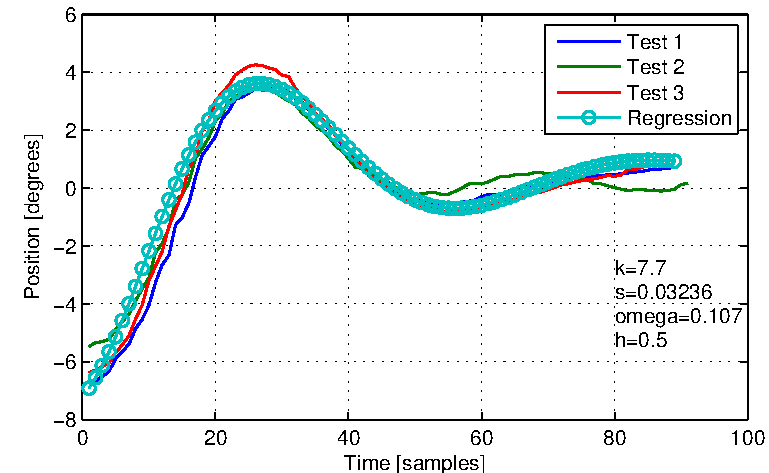
\includegraphics{plot/pbtest}
	\caption{Pitch test with Vicon, Bow pushed down.}
	\label{fig:pbtest}
\end{figure}
\begin{figure}[H]
	\centering
	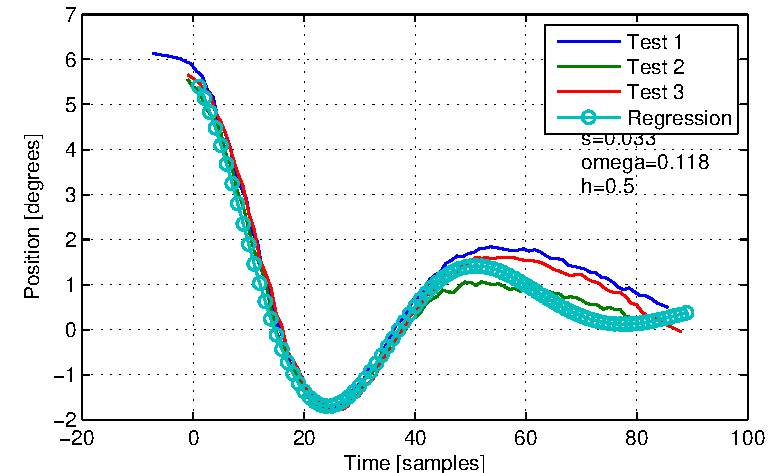
\includegraphics{plot/pstest}
	\caption{Pitch test with Vicon, Stern pushed down.}
	\label{fig:pstest}
\end{figure}

\newpage
\subsubsection{Roll test}
\begin{figure}[H]
	\centering
	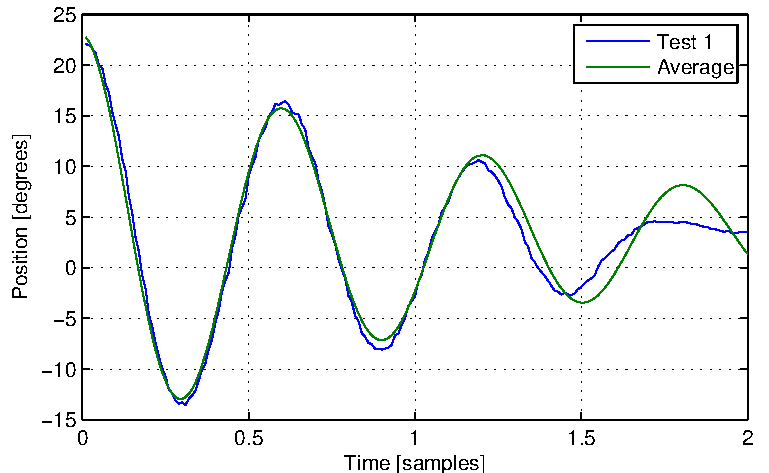
\includegraphics{plot/rltest}
	\caption{Roll left test with Vicon, Port side pushed down.}
	\label{fig:rltest}
\end{figure}
\begin{figure}[H]
	\centering
	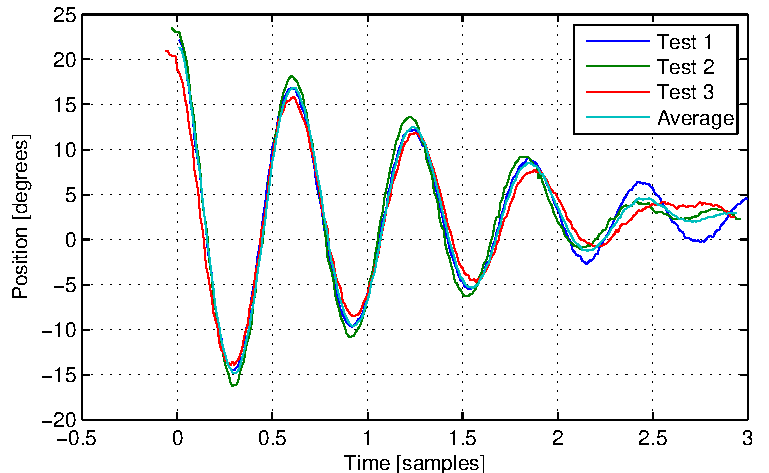
\includegraphics{plot/rrtest}
	\caption{Roll right test with Vicon, Starboard side pushed down.}
	\label{fig:rrtest}
\end{figure}


The rigid body constants for the vessel can be found in table \ref{tab:constants} and the results from measurements and estimation can be found in table \ref{tab:dmatrix}.
\todo{Disse skal måles op og sættes ind}
\begin{table}[htbp]
\centering
\begin{tabular}{ccc}
	\toprule
  Coefficient & Value \\
  \midrule
  $m$ & 2 \\
  $x_g$ & 2 \\
  $z_g$ & 2\\
  $I_{xz}$ & 2 \\
  $I_z$ & 2 \\
  $I_y$ & 2 \\
  $I_x$ & 2 \\
  $I_{zx}$ & 2 \\
  \bottomrule
\end{tabular}
\caption{Rigid body mass matrix constants for $M_{RB}$}
\label{tab:constants}
\end{table}

\begin{table}[htbp]
\centering
\begin{tabular}{ccc}
	\toprule
  Hydrodynamic\\Coefficient & Value \\
  \midrule
  $X_u$ & 2.86 \\
  $Y_v$ & 2 \\
  $K_v$ & 2 \\
  $N_v$ & 2 \\
  $N_r$ & 2 \\
  $Y_r$ & 2 \\
  $K_r$ & 2 \\
  $Y_p$ & 2 \\
  $K_p$ & 0.1677 \\
  $N_p$ & 2 \\
  $M_q$ & 0.8497 \\
	\bottomrule
\end{tabular}
\caption{Results of fitted values and the calculated coefficients.}
\label{tab:dmatrix}
\end{table}

\begin{table}[htbp]
\centering
\begin{tabular}{ccc}
	\toprule
  Restoring force\\Coefficient & Value \\
  \midrule
  $K_\varphi$ & 0.1385 \\
  $M_\theta$ & 0.1788 \\
  	\bottomrule
\end{tabular}
\caption{Results of fitted values and the calculated coefficients.}
\label{tab:gmatrix}
\end{table}

This makes the linear damping matrix as:
\begin{align}
D = -
\begin{bmatrix}
X_u & 0 & 0 & 0 & 0\\
0 & Y_v & Y_p & 0 & Y_r\\
0 & K_v & 0.1677 & 0 & K_r\\
0 & 0 & 0 & 0.8497 & 0\\
0 & N_v & N_p & 0 & N_r
\end{bmatrix}
\end{align}
and the restoring for matrix as:
\begin{align}
G = -
\begin{bmatrix}
0 & 0 & 0 & 0 & 0\\
0 & 0 & 0 & 0 & 0\\
0 & 0 & 0.1385 & 0 & 0\\
0 & 0 & 0 & 0.1788 & 0\\
0 & 0 & 0 & 0 & 0
\end{bmatrix}
\end{align}
and the rigid body matrix as:
\begin{align}
M_{RB} =
\begin{bmatrix}
m & 0 & 0 & mz_g & -my_g\\
0 & m & -mz_g & 0 & mx_g\\
0 & -mz_g & I_x & -I_{xy} & -I_{xz}\\
mz_g & 0 & -I_{yx} & I_y & -I_{yz}\\
-my_g & mx_g & -I_{zx} & -I_{zy} & I_z
\end{bmatrix}
\end{align}
\section{Discussion}


\section{Conclusion}

